\documentclass{llncs}

\usepackage{listings}
\usepackage{csquotes}
\usepackage{color}
\usepackage{caption}
\usepackage{graphicx}
\usepackage{oz}
\DeclareGraphicsExtensions{.pdf,.png,.jpg}
 \usepackage{listings}
 \usepackage{courier}
 \lstset{
         basicstyle=\footnotesize\ttfamily, % Standardschrift
         %numbers=left,               % Ort der Zeilennummern
         numberstyle=\tiny,          % Stil der Zeilennummern
         %stepnumber=2,               % Abstand zwischen den Zeilennummern
         numbersep=5pt,              % Abstand der Nummern zum Text
         tabsize=2,                  % Groesse von Tabs
         extendedchars=true,         %
         breaklines=true,            % Zeilen werden Umgebrochen
         keywordstyle=\color{red},
    		frame=b,         
 %        keywordstyle=[1]\textbf,    % Stil der Keywords
 %        keywordstyle=[2]\textbf,    %
 %        keywordstyle=[3]\textbf,    %
 %        keywordstyle=[4]\textbf,   \sqrt{\sqrt{}} %
         stringstyle=\color{white}\ttfamily, % Farbe der String
         showspaces=false,           % Leerzeichen anzeigen ?
         showtabs=false,             % Tabs anzeigen ?
         xleftmargin=17pt,
         framexleftmargin=17pt,
         framexrightmargin=5pt,
         framexbottommargin=4pt,
         %backgroundcolor=\color{lightgray},
         showstringspaces=false      % Leerzeichen in Strings anzeigen ?        
 }
 \lstloadlanguages{
         Java
 }
%\DeclareCaptionFont{blue}{\color{blue}} 

 %\captionsetup[lstlisting]{singlelinecheck=false, labelfont={blue}, textfont={blue}}
 % \usepackage{caption}
 
\DeclareCaptionFont{white}{\color{white}}
\DeclareCaptionFormat{listing}{\colorbox[cmyk]{0.43, 0.35, 0.35,0.01}{\parbox{\textwidth}{\hspace{15pt}#1#2#3}}}
 % \captionsetup[lstlisting]{format=listing,labelfont=white,textfont=white, singlelinecheck=false, margin=0pt, font={bf,footnotesize}}
 
    \graphicspath{{figs/}}
 


\captionsetup[lstlisting]{format=listing,labelfont=white,textfont=white, singlelinecheck=false, margin=0pt, font={bf,footnotesize}}




% we define a set of macros for constants of type 'Kind' 

\def\datamodel{\mathsf{datamodel}}
\def\dataclass{\mathsf{dataclass}}
\def\dataelement{\mathsf{dataelement}}
\def\enum{\mathsf{enum}}
\def\enumeration{\mathsf{enumeration}}
\def\primitivetype{\mathsf{primitivetype}}
\def\datatype{\mathsf{datatype}}

% and for multiplicity 

\def\optional{0{\upto}1}
\def\mandatory{1{\upto} 1}
\def\many{0{\upto}*}

% our partial ordering on constraints

\def\Cimplies{\mathrel{\implies_c}}
\def\Ciff{\mathrel{\iff_c}}

% our partial ordering on text (this will become interesting later)

\def\Timplies{\mathrel{\implies_t}}
\def\Tiff{\mathrel{\iff_t}}

% and conjunction 

\def\Tand{\mathrel{\land_t}}
\def\TAnd{\mathop{\land_t}}

% our globalised version of the defining relations

\def\refines{\mathrel{refines}}
\def\newVersionOf{\mathrel{newVersionOf}}
\def\extends{\mathrel{extends}}
\def\contains{\mathrel{contains}}

% we may have \sqsubseteq and \gg when it comes to analysis 

% our two status values 

\def\draft{\mathsf{draft}}
\def\final{\mathsf{final}}

\usepackage{zed}

\begin{document}

\title{Formal Specification to Model Based Engineering}
%If Title is too long, use \titlerunning
%\titlerunning{Short Title}

%Single institute
\author{Jim Davies, David Milward \and Seyyed Shah}
%If there are too many authors, use \authorrunning
%\authorrunning{First Author et al.}
\institute{University of Oxford}
\maketitle

\begin{abstract}
In this paper we present an ISO11179 metadata registry using a data-oriented Domain Specific Modelling Language (DSML). In particular we examine how certain aspects of the ISO11179 specification can be strengthened by using a specific DSML built to handle interoperability use cases, and also how using a model based engineering framework addresses ambiguities in the standard. We examine how the DSML approach taken in this paper presents a concrete realisation of data componentisation, harmonisation, standardisation and reuse of meta-data components. We also examine how the ISO11179 based DSML can be implemented using the Eclipse Modelling Framework and made interoperable with UML In particular, we identify how Model Driven Engineering has helped in achieving the specific goals of ISO11179 via a case study.

\end{abstract}

\keywords{...}
\noindent

\section{Introduction}

\section{Design of an ISO11179 Metadata Registry}

The ISO11179 standard as discussed describes a metamodel using text and UML 2.4. In order to arrive at a working model based specification we have taken that description and written it using a formal specification language.  This enabled us to generate both the registry and some of the transformations required to express datasets in terms of the standard.  ISO11179-3 has a detailed account of the registry metamodel and its attributes, and sets out to be relevent to application designers, system architects, and software developers. It uses UML 2.4.1 as a modelling language to describe the main features of a conformant metadata registry, although the standard itself is quite clear in not endorsing any particular environment, database management system, database design paradigm, system development methodology, data definition language, command language, system interface, user interface, computing platform or technology required for implementation. However in ISO11179-3.5 a metamodel is used to describe the information model of a metadata registry, and again the standard is clear that this should not limit the actual implementation technology used. The UML description is split into a number of packages:
\begin{itemize}
\item Basic Package
\item Identification Metamodel
\item Designation and Definition Metamodel
\item Registration Package
\item Concepts Package (Concepts and Classification regions)
\item Binary Relations Package
\item Data Descriptions Package
\end{itemize}

The standard continues to provide a detailed account of how metadata items are related within the metadata registry, for the purposes of brevity we will not repeat them all here, but we may refer back to specific parts of the standard where required.

This section details a brief account of the specification of the ISO11179 registry which was carried out using Z. From the resulting Z specification we have built the DSML on which we have built the metadata registry. The metadata registry has then been used for the creation, curation and management of a variety of datasets which we detail in the Results section. 

The metamodel or language for data we describe is informed by our experience with Healthcare information systems which is documented in a previous paper \cite{DSMCR} and by the development of an open source Metadata Registry built around similar principles. The DSML has been built to help with data curation and creation in the Healthcare domain, and as such is the result of discussion with domain experts in this sector. The reason for designing this DSML is that we seek a meta-language to be able handle hetrogeneous metadata stored using a variety of languages. It needs to be able to capture metadata, in particular a detailed description the data is stored in relational databases, XML Schemas, XML files based on XML Schemas, Excel files and object-oriented programs. It then needs to be able to automatically transform the data into a number of simple formats. To do this each dataset at an M1 level needs to be described at the M2 level, by doing this we can build a container which can hold the metadata collected at the M1 level.

The metamodel in ISO11179-3 is defined in terms of UML and text, and the description is split into a number of packages, which we review in brief.
\begin{zed}
[Packages,basicPackage, IdentificationMetamodel, \\
DesignationAndDefinitionMetamodel,RegistrationPackage, \\
ConceptsPackage, BinaryRelationsPackage, DataDescriptionsPackage]

\end{zed}

ISO11179-3sect1 describes the scope of the documents, and states that sections 5-11 form a specification of a \emph{Platform Independent Model} for a metadata registry. Section 12 describes basic attributes for metadata items in a situation where a full metadata registry implementation is not available or possible. Section 2 deals with normative references, the only indispensible referenced document listed is ISO11179-6. Section 3 introduces terms, we will make reference to this section where needed in the course of this specification.Section 4 deals with conformance and is not directly relevent to the work here.

We start with section 5 which details the overview of the packages involved with the MDR, indeed it is described as a metamodel for the infomraiton model of a MDR. This metamodel is terms the \emph{Registry Metamodel} and is specified as a \emph{conceptual data model - one that describes how relevant information is structured in the natural world, in other words how the human mind is accustomed to thinking of the information}. It must be observed that the previous statement is factually incorrect and demonstrates the enormous arrogance of the ISO11179 committee members, who demonstrate very little understanding of current neuro-science, especially recent insights into how the human mind is or is not accustomed to handling information, the only reason to continue with this twaddle is to demonstrate once and for all what an inadequate document it is.

Section 5 continues by stating that there is no one-to-one match between attributes of the metamodel and fields, columns or other database artefacts, and it emphasises the fact that the physical implementation may or may not be distributes, implemented using databases, XML, RDF/OWL or any other related information processing systems. However it does go on to state that minimum and maximum constraints of attributes should be enforced at all times, and that constraints on minimum occurences are to be enforced when the registration status of the metadata item is "recorded" or higher. It would seem that the latter statement is overruled by the former statement, so it is ignored for this specification.

The standard uses the term \emph{metamodel construct} to refer to the UML model constructs or artefacts being used, and \emph{metadata object} for the model being specified, UML 2.4.1 is used in the version being examined. The metamodel is split into six packages and the dependencies between them are illustrated in Figue ~\ref{fig:pack}, some are further subdivided into "regions" (although this is not a formal UML term).

\begin{figure}[h]
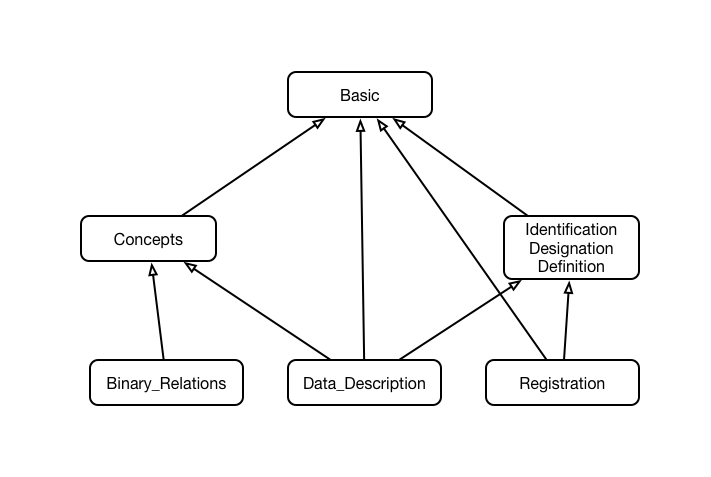
\includegraphics[width=1.0\textwidth,natwidth=610,natheight=642]{ISOPack}
\caption{Data Description Model} 
\label{fig:pack}
\end{figure}

There are 3 types of dependency listed : subclassing between packages, relationships and referenced datatypes.

A metadata item may be "extended by" any one of six related stereotypes, based on classes which are covered in later sections, they are \emph{Identified\_Item}, \emph{Registered\_Item},\emph{Administered\_Item},\emph{Attached\_Item},\emph{Designatable\_Item},\emph{Classifiable\_Item}.
\begin{zed}
[Scoped\_Identifier,metadataItem,Designation,Definition,Concept,Submisson\_Record,\\
Stewardship\_Record,Registration\_Authority,Administered\_Record]
\end{zed}

\begin{schema}{IdentifiedMetaDataItem}
identification\_association: metadataItem \pfun Scoped\_Identifier \\
\where
 \#identification\_association \leq 1 \\
\end{schema}

\begin{schema}{DesignatedMetaDataItem}
item\_designation\_association: metadataItem \pfun Designation \\
\where
 \#item\_designation\_association \leq 1 \\
\end{schema}

\begin{schema}{DefinedMetaDataItem}
item\_definition\_association: metadataItem \pfun Definition \\
\where
 \#item\_definition\_association \leq 1 \\
\end{schema}

\begin{schema}{ConceptMetaDataItem}
classification\_association: metadataItem \pfun Concept \\
\where
 \#classification\_association \leq 1 \\
\end{schema}

\begin{schema}{RegisteredMetaDataItem}
identification\_association : metadataItem \pfun Scoped\_Identifier \\
submission\_association : metadataItem \pfun Submisson\_Record \\
\where
 \#identification\_association \leq 1 \\
 \#submission\_association \leq 1 \\
\end{schema}

\begin{schema}{AdministeredMetaDataItem}
identification\_association: metadataItem \pfun Scoped\_Identifier \\
submission\_association: metadataItem \pfun Submisson\_Record \\
stewardship\_association: metadataItem \pfun Stewardship\_Record \\
registration\_association: metadataItem \pfun Registration\_Authority \\
attachment\_association: metadataItem \pfun Administered\_Record \\
\where
 \#stewardship\_association\leq 1 \\
 \#registration\_association \leq 1 \\
 \#attachment\_association = 0 \\
 \#identification\_association \leq 1 \\
\end{schema}

\begin{schema}{AttachedMetaDataItem}
stewardship\_association: metadataItem \pfun Stewardship\_Record \\
attachment\_associations: metadataItem \pfun Administered\_Record \\
\where
 \#attachment\_associations \leq 1 \\
 \#stewardship\_association = 0 \\
\end{schema}


A metadataItem may be extended with \emph{Slots} which allow the metadataItems to be extended with custom attributes, relationships, classes and even complete new packages.
\begin{zed}
[String]
\end{zed}
\begin{schema}{Slot}
  key: \nat \\
  value: String \\
\end{schema}

\begin{schema}{ExtendedMetaDataItem}
	slot\_association: metadataItem \pfun Slot \\
\where
 	\#slot\_association \geq 0 \\
\end{schema}

  

\subsection{ISO11179:3 Basic Package}

This section introduces a number of basic types, some of which are already defined in Z (Boolean, Integer and Natural Range - or Natural Number), the others we can introduce as follows:
\begin{zed}
[ Date, Value, Sign, PostalAddress, Datetime,  Text,Notation, PhoneNumber]
\end{zed}
This section introduces the basic types, together with a number of classes: ReferenceDocument, DocumentType, Contact RegistrationAuthorityIdentifier, Individual, LanguageIdentification, Role, Organization.


\subsubsection{Classes overview}

\begin{class}{Language\_Identification}
\also
language\_identifier : String \\
script\_identifier : String \\
geopolitical\_territory\_identifier : String \\
variant\_identifier: Notation \\
extention\_identifier : String\\
private\_use\_qualifier: String\\
\end{class}

\begin{class}{Reference\_Document}
\also
identifier : String \\
document\_type : Document\_Type \\
language : Language\_Identification \\
notation: Notation \\
title : Text\\
provider: Organization\\
url: String
\end{class}



\begin{class}{Document\_Type}
\also
identifier : String \\
description : Text \\
scheme\_reference : Sign \\
\end{class}

\begin{class}{Registration\_Authority\_Identifier}
\also
international\_code\_designator : String \\
organizational\_identifier : String \\
organizational\_part\_identifier: Document\_Type \\
OPI\_source : String \\
\end{class}

\begin{class}{Role}
\also
title : Sign \\
mail\_address : Postal\_Address \\
email\_address : String \\
phone\_number: Phone\_Number \\
\end{class}

\begin{class}{Contact}
\also
individual : Individual \\
organization : Organization \\
role : Role \\
\end{class}

\begin{class}{Individual}
\also
name : Sign \\
title : Sign \\
mail\_address : Postal\_Address \\
email\_address : String \\
phone\_number: Phone\_Number \\
role : Role \\
\end{class}

\begin{class}{Organization}
\also
name : String \\
mail\_address : Postal\_Address \\
email\_address : String \\
phone\_number: Phone\_Number \\
uri : String\\
\end{class}




\subsection{ISO11179:3 Identification Metamodel }
Here the subject of how to uniquely identify a metadata item is discussed, so classes of Namespace, ScopedIdentifier, IdentifiedItem and Slot are introduced.

\begin{zed}
  [Item, ScopedId, Organization, Namespace, Name, Term, Id]
\end{zed}
\begin{zed}
  Path == \seq Name \\
\end{zed}


The standard describes in detail that each identified item needs to have a scoped identifier, which in turn is unque within a particular namespace. A namespace is a unque name, which is used as part of a reference scheme, it is normally a URL such as : \emph{http://www.dictionary.com}. In terms of the specification we can describe a namespace simply as a sequence of Names (with a few other properties), and so a Scoped\_Identifier becomes relation between an identifier and namespace. This is shown in the IdentifiedItem schema below: 


\begin{schema}{IdentifiedItem}
  item : ScopedId \pfun Item \\
  scopedId : Id \pfun Path \\
  slot: Item \pfun Slot
\end{schema}

We've added in the slot reference, however this is not relevant for identification discussion at present.

\subsubsection{ISO11179:3 Designation and Definition Metamodel}

A DesignatableItem is one which can have zero to many description(s) or designation(s), in a particular language, and one which can have zero to many definitions, again these can be in various languages. Here the idea of a \emph{sign} is a replacement term for \emph{name}, extended to encompass the use of a accronym or icon to identify the item.
\begin{schema}{DesignatableItem}
  designation : Sign \pfun Item \\
  definition : Text \pfun Item \\
\end{schema}



\subsubsection{ISO11179:3 Registration Package}

The registration package supports registration of a metadata item by an authorised person. 

A RegisteredItem is an IdentifiedItem, it may also be a DesignatedItem and it may also be a Classifiable item. It can be either an AdministeredItem or an AttachedItem.


\begin{zed}
[LanguageTag]
\end{zed}
\begin{schema}{AdministeredItem}
changeDescription : Text \\
creationDate : Datetime \\
lastChangeDate : Datetime\\

\end{schema}

\begin{schema}{AttachedItem}
itemId: Id \\
ownedBy : Id
\end{schema}
 
\begin{zed}
RegisteredItem ::=  ad\ldata AdministeredItem \rdata |at\ldata AttachedItem \rdata
\end{zed}


\subsubsection{Concepts Package}
The purpose of the concepts package is to describe concepts and the various relations which hold between concepts, \emph{Ontologies} are supported by Concept\_Systems and Assertions. A \emph{concept} is a unit of knowledge created by a unique combination of characteristics. The standard mandates that a concept must be a member of at least one \emph{Concept\_System}, and that each \emph{Concept\_System} will act as the \emph{source} of each \emph{concept}. A concept system is a container of concepts which can be related by relations. A \emph{Concept\_System} will be described by on \emph{notation} attribute which is used to describe it. The \emph{notation} is defined as the formal syntax and semantics used in the  \emph{Concept\_System}, an example of which is given as OWL-DL XML notation, or XCL Common Logic.

A \emph{Concept} can have zero to many \emph{Assertions} which are propositional sentences describing something that can be asserted. An Assertion must also have one or more \emph{Relations}, one or more \emph{Concepts} and be included in one or more \emph{Concept\_Systems}

A \emph{Classifiable\_Item} is an item which may be classified into a hierarchical structure or partial order. This is accomplished by associating it with one or more \emph{Concepts}, which can optionally be associated with a \emph{Classification}. 

\subsubsection{Binary Relations Package}
The binary relations package attempts to model various aspects of relations in a UML class diagram. The Binary\_Relation class is derived from the Relation class, and has attributes of reflexivity, Symmetry and Transitivity, each of which are modelled by separate classes. In Z Binary relations are built into the language, and so many of the properties listed may be expressed more easily using Z.

\subsubsection{Data Description Package}
This package is probably the most important in the standard because it details how the metadata registry should handle the core data, in short how data held in the registry needs to be described. However it is also the most difficult, and writing the specification resulted in a number of potential ambiguities which arise from the fact that the description provides both text and UML to describe the package, using UML implies that the description is at the M1 level, however it is not since we are describe how to store metadata, in short we are describing metadata. This puts the description firmly in the M2 or meta-meta-language abstraction level, which means a direct translation of the UML class diagrams to code is not what is intended in this standard.

The start of the section describes a high-level set of relationships between the following classes: Data\_Element\_Concept, a Conceptual\_Domain, a Data\_Element and a Value\_Domain. 





If we introduce some of these items:

A \emph{Data\_Element\_Concept} class is a class which models a data element concept, which is a concept that is an \emph{association} of a property and an object class. In Z we can model an association as a relation and this states that:

\begin{zed}
[Property,  ObjectClass, dataElement, valueDomain, \\
		 valueMeaning,  concept, conceptualDomain] \\
		 dataElementConcept == Property \pfun ObjectClass\\
\end{zed}
We can then identify some of the relations between them:

\begin{zed}
dataElementConceptDomain == dataElementConcept \pfun conceptualDomain\\
dataElementMeaning == dataElement \pfun dataElementConcept\\
dataElementValueDomain == dataElement \pfun valueDomain \\
valueDomainMeaning == valueDomain \pfun conceptualDomain \\
\end{zed}



There are some details which are hard to represent, for instance the fact that a \emph{Conceptual\_Domain} is described by a UML class which is a child class of \emph{Concept} and also is given the definition in text that it is a \emph{set of value meanings}. Value meanings are also decribed as sub-types of the class \emph{Concept} in this section, however no real account of the differences of the various sub-types of \emph{Concept} are provided.  A conceptual domain can facilatate the mapping of equivalent values of two or more value domains. It might also be used in several \emph{value domains} that share the \emph{conceptual domain}. In the standard this is explained with reference to ISO3166 the standard for country codes, so the \emph{conceptual domain} is \emph{countries of the world}. The three letter and two letter codes in ISO3166 are therefore different value domains. The standard then goes on to explain that a conceptual domain may be used by several \emph{data element concepts} for example, a person's country of citizenship, a persons country of residence and a person's country of birth. 

A value domain is a collection of permissible values, it provides representation for a data element concept, but provides no implication over meanings or associations. Permissible values are designations or bindings of signs to their corresponding value meanings. The idea of a datatype is introduced in this section, but as an attribute of a value domain, together with the idea of a \emph{unit\_of\_measure}, a \emph{format}, and a \emph{maximum\_character\_quality}. Value meaning is defined as \emph{``semantic content of possible values''}, so we can interprete a  \emph{Conceptual\_Domain} as being a set of semantics of possible values. In the example given we see that the semantics of a \emph{Conceptual\_Domain} is given by the relations between the \emph{Conceptual\_Domain}, in this case \emph{Country} and the \emph{Person}.

An example of a conceptual domain and a set of value domains is ISO3166, whereby the conceptual domain is the names of countries which has 7 different value domains, one for each representation (short French, Short English, etc).  A Value domain shall participate in the association: a value\_domain\_meaning in exactly one \emph{Conceptual\_Domain} provides meaning to the value domain. Elsewhere the standard defines value domains as collections of mappings between value meanings and values.

A \emph{Data\_Element} is a class which models a data element, which is an atomic unit of data, an example of which could be a column in a database table, or a field in a record, or an attribute of a java class.




\
An \emph{Object Class} is described as being a \emph{concept} that represents a set of ideas, abstractions or things in the real world that can be identified with explicit boundaries and meaning. We interprete this is as being the same as the notion of \emph{Class} in the MBE world. It is one of the only entities which is able to collect, contain or group data elements, the other entity that is able to group elements is a Classification.

The specification is over 240 pages long, and this section 11 is over 15 pages so rather than list the specification here we describe the main aspects on which the DSML has been based. The data description package describes the way in which the concepts behind the data are mapped, however many of the ideas contained here are relevent to and concern themselves with aspects of the conceptual model which cannot be derived automatically from a dataset.   Also by further analysis of the Identification specification we find that one of the easiest ways to identify and version data elements is using the a series of paths or strings which identify the \emph{group} which the data element is a component of. This feature makes \emph{Model} a first class entity in our metadata registry design



\begin{figure}[h]
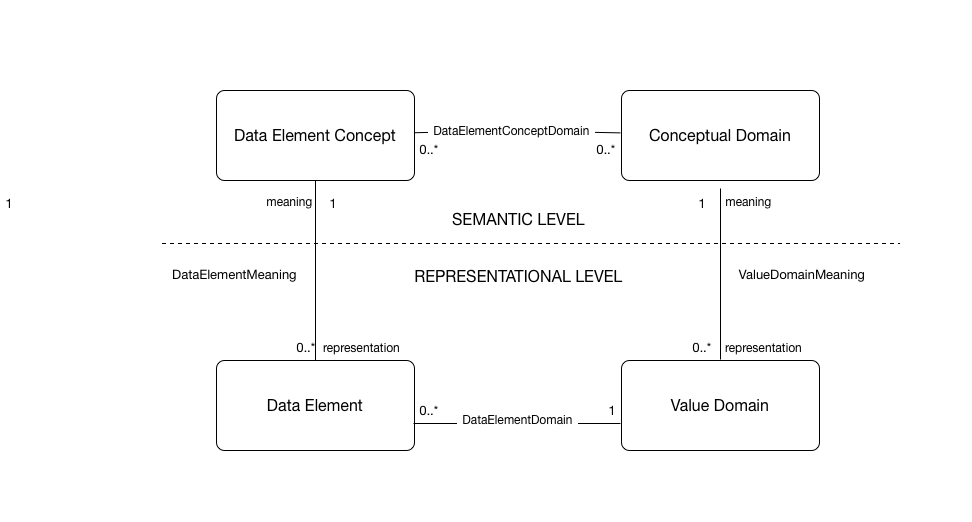
\includegraphics[width=1.0\textwidth,natwidth=610,natheight=642]{DataDescModel}
\caption{Data Description Model} 
\label{fig:ddmodel}
\end{figure}

\begin{class}{Data\_Element\_Concept}


 \end{class}
 


\newpage


\bibliographystyle{plain}

\bibliography{objZ2ocl}

\end{document}

